\subsection{Joint vs Disjoint}\label{sec:joint-vs-disjoint}
Here we want to compare the joint and disjoint solutions.
For this comparison we use two different topology to have better insights and fair results.

\subsubsection{FatTree}
Here we will use FatTree topology with k equals to 6.
As you can see results confirm our hypothesis that joint solutions makes better revenues.

\begin{table}[H]
    \caption{Revenues from Joint and Disjoint Solutions on FatTree Topology with k equals to 6}
    \label{tbl:joint-vs-disjoin-fattree}
    \medskip
    \centering
    \begin{tabular}{lrrr}
        \toprule
        {} &    joint &  disjoint &  nchains \\
        \midrule
        0 &  45440.0 &   44980.0 &      100 \\
        1 &  36660.0 &   17090.0 &       80 \\
        2 &  27850.0 &   13340.0 &       60 \\
        3 &  18340.0 &   13440.0 &       40 \\
        4 &   9170.0 &    1880.0 &       20 \\
        \bottomrule
    \end{tabular}
\end{table}

\begin{figure}[H]
    \centering
    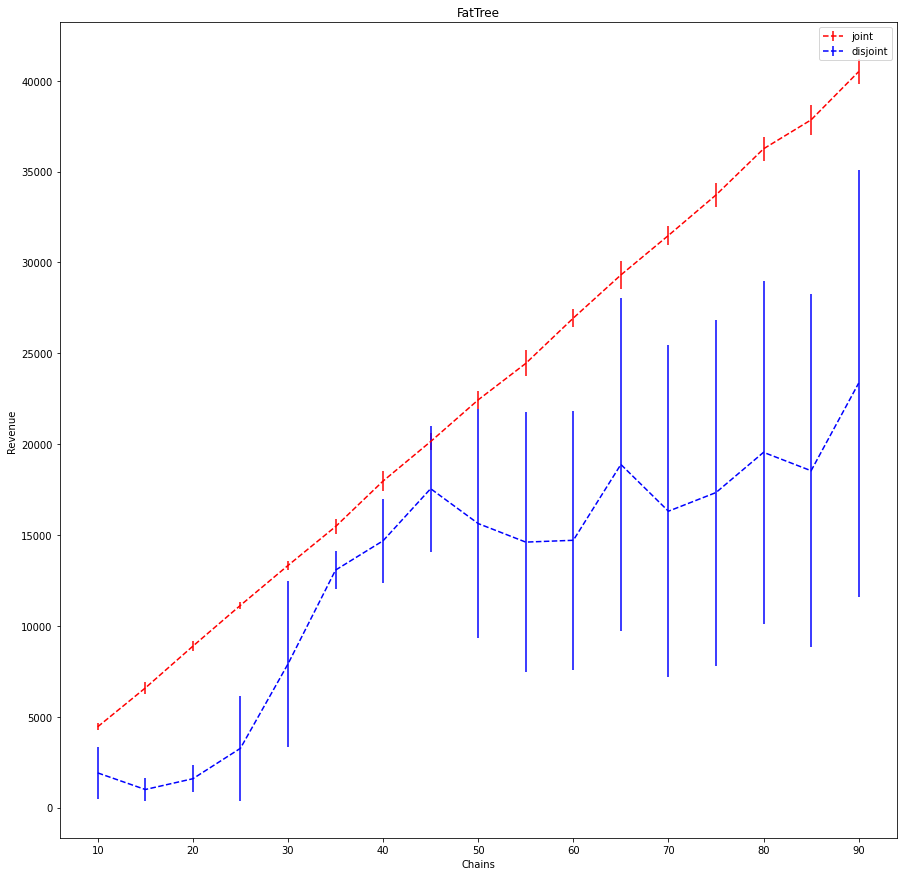
\includegraphics[height=350pt]{plots/joint-vs-disjoint-fattree.png}
    \caption{Revenues from Joint and Disjoint Solutions on FatTree Topology with k equals to 6}
    \label{fig:joint-vs-disjoint-fattree}
\end{figure}

\subsection{USNet}
Here we will use USNet topology with 3 to 4 nodes attached to each of its points.
As you can see the results show joint and disjoint solutions on this setup work equally because there is no specific
management requirement and topology can handle all chains.

\begin{table}[H]
    \caption{Revenues from Joint and Disjoint Solutions on USNet Topology}
    \label{tbl:joint-vs-disjoin-usnet}
    \medskip
    \centering
    \begin{tabular}{lrrr}
        \toprule
        {} &    joint &  disjoint &  nchains \\
        \midrule
        0 &  23000.0 &   23010.0 &       50 \\
        1 &  34180.0 &   34260.0 &       75 \\
        2 &  45430.0 &   45560.0 &      100 \\
        3 &  57180.0 &   57380.0 &      125 \\
        4 &  68750.0 &   69360.0 &      150 \\
        \bottomrule
    \end{tabular}
\end{table}

\begin{figure}[H]
    \centering
    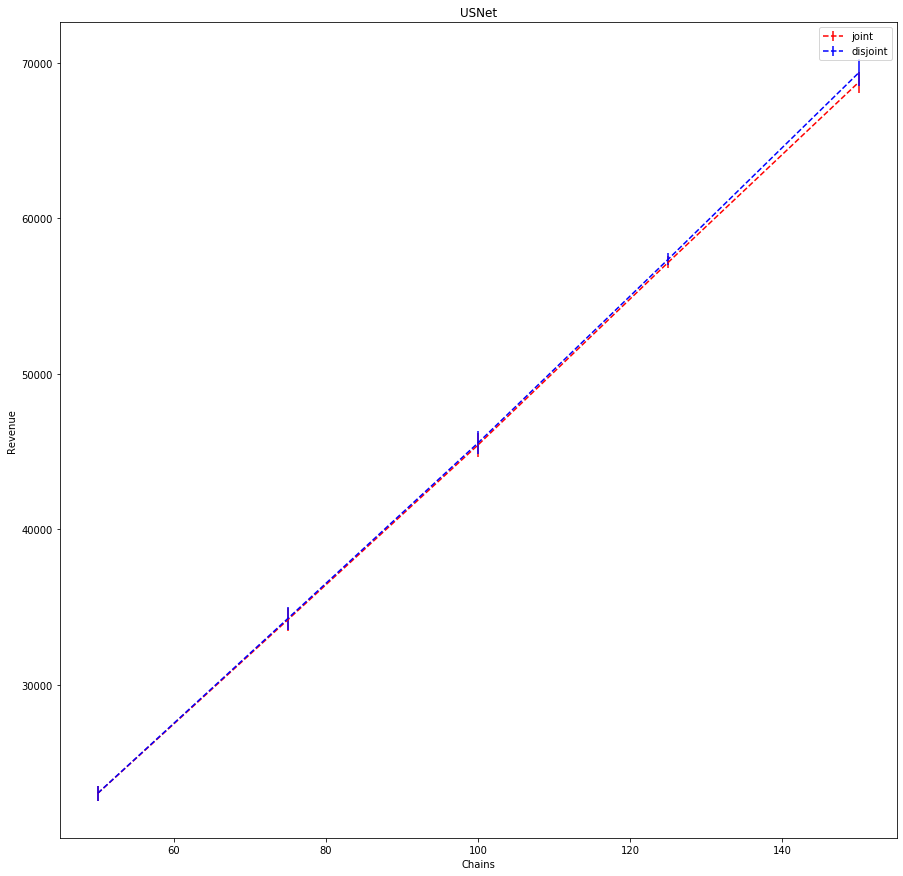
\includegraphics[height=350pt]{plots/joint-vs-disjoint-usnet.png}
    \caption{Revenues from Joint and Disjoint Solutions on USNet Topology}
    \label{fig:joint-vs-disjoint-usnet}
\end{figure}
